Recurrent Neural Network (RNN) là một mô hình mạng neural hồi quy gồm 3 thành phần chính là Input layer, Hidden layer và Output layer.

Mô hình tổng hợp và lan truyền thông tin theo trình tự xâu chuỗi. Mô hình được gọi là hồi quy vì thực hiện tính toán ở thời điểm hiện tại sẽ phụ thuộc vào các kết quả tính toán ở những thời điểm trước đó. Do đó, RNN phải nhớ thông tin đã được đưa vào để tính toán trước đó để phục vụ cho các bước tính toán sau này.

Sau nhiều bước biến đổi, các thông tin ở những bước đầu tiên bị biến đổi nhiều lần dẫn đến bị triệt tiêu. Do đó, RNN chỉ có nhớ được một vài bước trước đó để mô hình được tối ưu nhất.

\begin{figure}[htbp]
\centerline{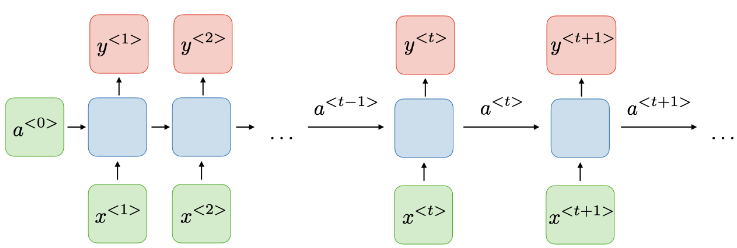
\includegraphics[width=0.4\textwidth]{img/RNN.png}}
\caption{Kiến trúc RNN}
\label{fig}
\end{figure}

RNN được biểu diễn bằng công thức sau:
\begin{align}
    a^{<t>} &= g_1(W_{aa}a^{<t-1>} + W_{ax}x^{<t>} + b_a) \\
    y^{<t>} &= g_2(W_{ya}a^{<t>} + b_y)
\end{align}

Trong đó:
\begin{itemize}
    \item $x^{<t>}$: giá trị đầu vào tại thời điểm $t$
    \item $y^{<t>}$: giá trị đầu ra tại thời điểm $t$
    \item $a^{<t>}$: giá trị kích hoạt
    \item $W_{aa}, W_{ax}, W_{ya}$: các ma trận trọng số
    \item $b_a, b_y$: vector độ lệch
    \item $g_1, g_2$: các hàm kích hoạt
\end{itemize}